%%%%%%%%%%%%%%%%%%%%%%%%%%%%%%%%%%%%%%%%%%%%%%%%%%%%%%%%%%%%%%%%%%%%%%%%
\section{Profiling}
\label{sec:profiling}
%%%%%%%%%%%%%%%%%%%%%%%%%%%%%%%%%%%%%%%%%%%%%%%%%%%%%%%%%%%%%%%%%%%%%%%%

Figure \ref{fig:profile} shows the profiling output of object detection of a single image, using SSD and YOLO. Profiling was done using NVIDIA Visual Profiler.

One of Jetson's strengths is that its CPU and GPU share the same memory. Therefore, host-to-device (HtoD) and device-to-host (DtoH) copies can be optimized to zero-copy \cite{tegrazerocopy}. Zero-copy will have no effect on SSD and YOLO, since memory copies are not frequent, therefore, there is no speedup potential. In addition, there are no overlapping opportunities between HtoD, DtoH, and the compute kernels, since there are almost no memory copies.

In terms of compute intensity, both algorithms use 75\% of their compute time in cuDNN kernels. There is no parallelism between kernels. SSD and YOLO fetch and analyze each image in serial, so theoretically, one can analyze a couple of images in parallel. However, Jetson TX1 has only 2 SMs, with 128 CUDA cores each, therefore, adding additional threads to the system, or running two or more object detection processes in parallel, achieves no performance gains.

\begin{figure*}[t]
	\begin{center}
	\subfloat[SSD]{
		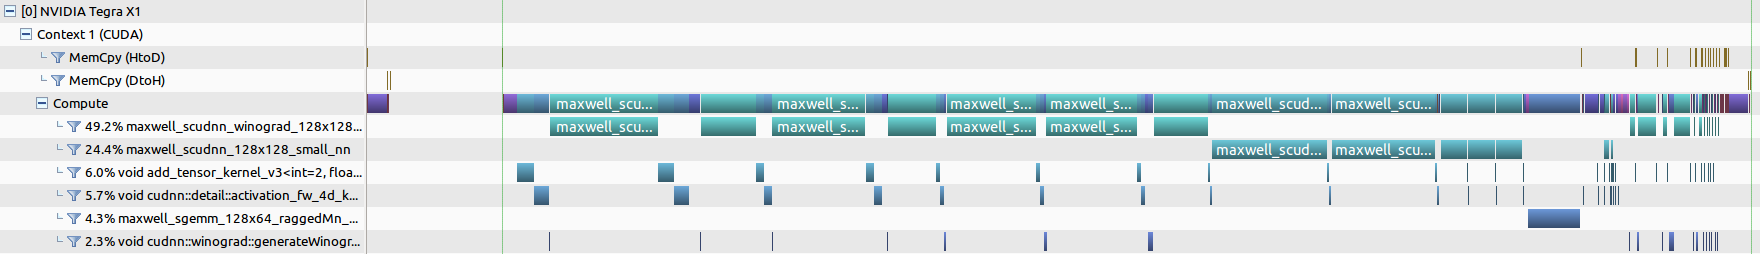
\includegraphics[width=1\textwidth]{./imgs/ssd-1frame.png}
		\label{fig:profile:ssd}
	} \\
	\subfloat[YOLO]{
		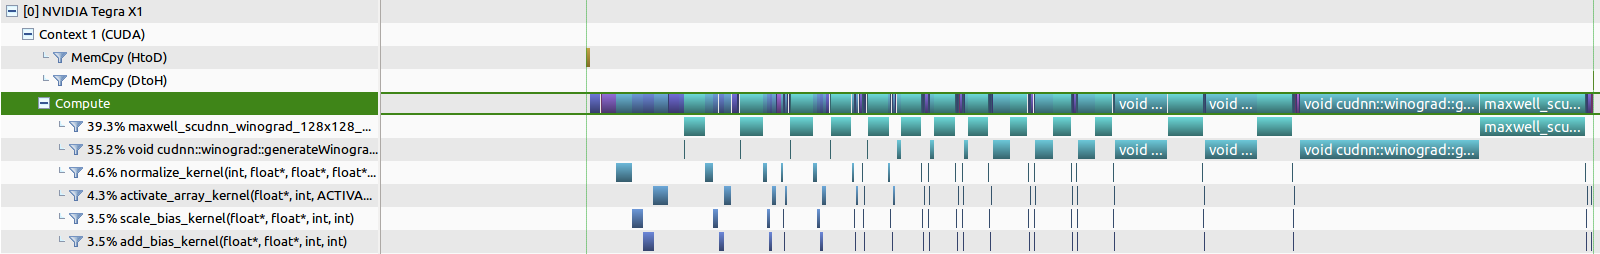
\includegraphics[width=1\textwidth]{./imgs/yolo-1frame.png}
		\label{fig:profile:yolo}
	}

	\caption{Profiling object detection on a single image with GPU and cuDNN on Jetson TX1, using NVIDIA Visual Profiler}
	\label{fig:profile}
	\end{center}
\end{figure*}


